\subsection{Before-ARC Schema}

A very frequent type of ARC task in the public training dataset can be labeled "conditional transform". It often consists in transforming some part of the grid with a very specific transformation, subject to a specific condition.  For instance, the training task \textit{db3e9e38} shown in Figure \ref{fig:conditional_transform_training} can be solved by cropping the grid to the only symmetric object of the grid. 

\begin{figure}[H] 
    \centering
    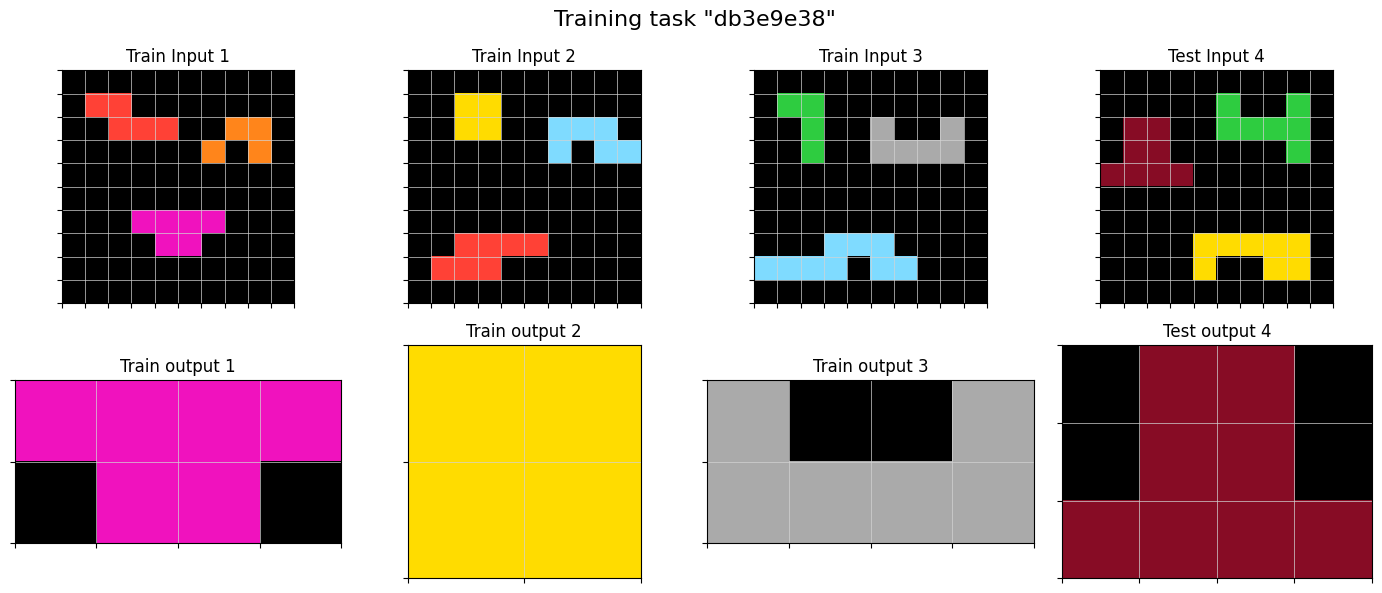
\includegraphics[width=0.8\columnwidth]{Figures/conditional_transform_example_training_example.png}
    \caption{Simple example of a "conditional transform like" task from the ARC training sample. Task ID: db3e9e38}
    \label{fig:conditional_transform_training}
\end{figure}

We chose to follow this logic scheme (which we call "conditional transform"). In this scheme, objects are positioned on a grid and a transformation is applied (or not) if a certain condition is satisfied. 

\subfile{objects.tex}

\subsubsection{Conditional Transform Algorithm}

Below is a simplified pseudo-code for the general algorithmic logic of the \texttt{ConditionalTransform} generator:

\begin{algorithm}
    \caption{\texttt{GenerateSingleTask(init\_params)} - Conditional Transform Schemata}
    \label{conditional_transform_algorithm}
    \begin{algorithmic}[1] % The number tells where the line numbering should start
        \State transform $\gets \texttt{sampleTransform}(\text{init\_params, possible\_transforms})$
        \State conditional $\gets \texttt{sampleConditional}(\text{init\_params, possible\_conditionals})$
        \While {trial\_n < 100 \ $\&$ \ example\_n $\leq$ wanted\_examples}
            \State input\_grid, objects $\gets \texttt{setInitialGrid}(\text{init\_params, transform, conditional})$
            \For {object in objects}
                \State output\_grid $\gets \texttt{position\_shape}(\texttt{transform\_shape}(\text{shape, transform}))$
            \EndFor
            \State task $\gets \text{(input\_grid, output\_grid)}$
        \EndWhile
        \State \textbf{Return:} task, transform, conditional 
    \end{algorithmic}
\end{algorithm}

The most critical function from this algorithm is \texttt{SetInitialGrid()}, which sets up the randomly sampled objects in the grid given the init\_params and the chosen transform and conditional. The objects and grid size must be initially set on the input grid in such a way that the transform and conditional can be applied without leading to invalidity, overdetermination or underdetermination (see below). Since we preferred allowing users to freely add their condition and transformations to the grid, we opted for a sampling solution, where initial grids are sampled and applying the transform and conditionals is attempted until a (seemingly) valid grid is reached. While this is less efficient than specifying all the constraints a given transform and condition are bound to in terms of initial grid arrangement, it allows more freedom to the user and still doesn't overcomplicate the algorithm. 

While the depth of conditional and transformation is limited to 1 (e.g. only a single transform and a single conditional can be combined to make a task rule), the user can easily extend the depth by providing new single transformations and conditionals which would be combination of other ones. For instance, if "translate\_shape\_up" is a transformation, and "rotate\_90" is another one, the user can easily create another transformation that would be the combination of the two: "translate\_shape\_up\_rotate\_90". This makes the generator ideal for studying compositionality - where models individually learning transformation A and transformation B can be tested at transformation AB. 

The user can specify the \textit{init\_params} such as grid\_size, min and max number of objects, specific transform and conditionals, max number of trials and more. There are in the current implementation a total of 15 transforms and 30 conditionals, making for a theoretical maximum of 450 distinct tasks. This number can easily be extended. 

On average, a single input output-pair is generated within 0.025 seconds, although this varies depending on several parameters, such as the grid size, transformation/conditional type, number of objects etc... This is due to varying failing frequency of applying rules depending on the initial grid configuration. 

and have transformation successfully applied if we have a small grid with multiple objects. The computation time also depends on the combination of transformation and conditionals to be applied - some combinations are more difficult to get right, and others are impossible - thereby maxing out the 100 trials. 

\begin{figure}[H] 
    \centering
    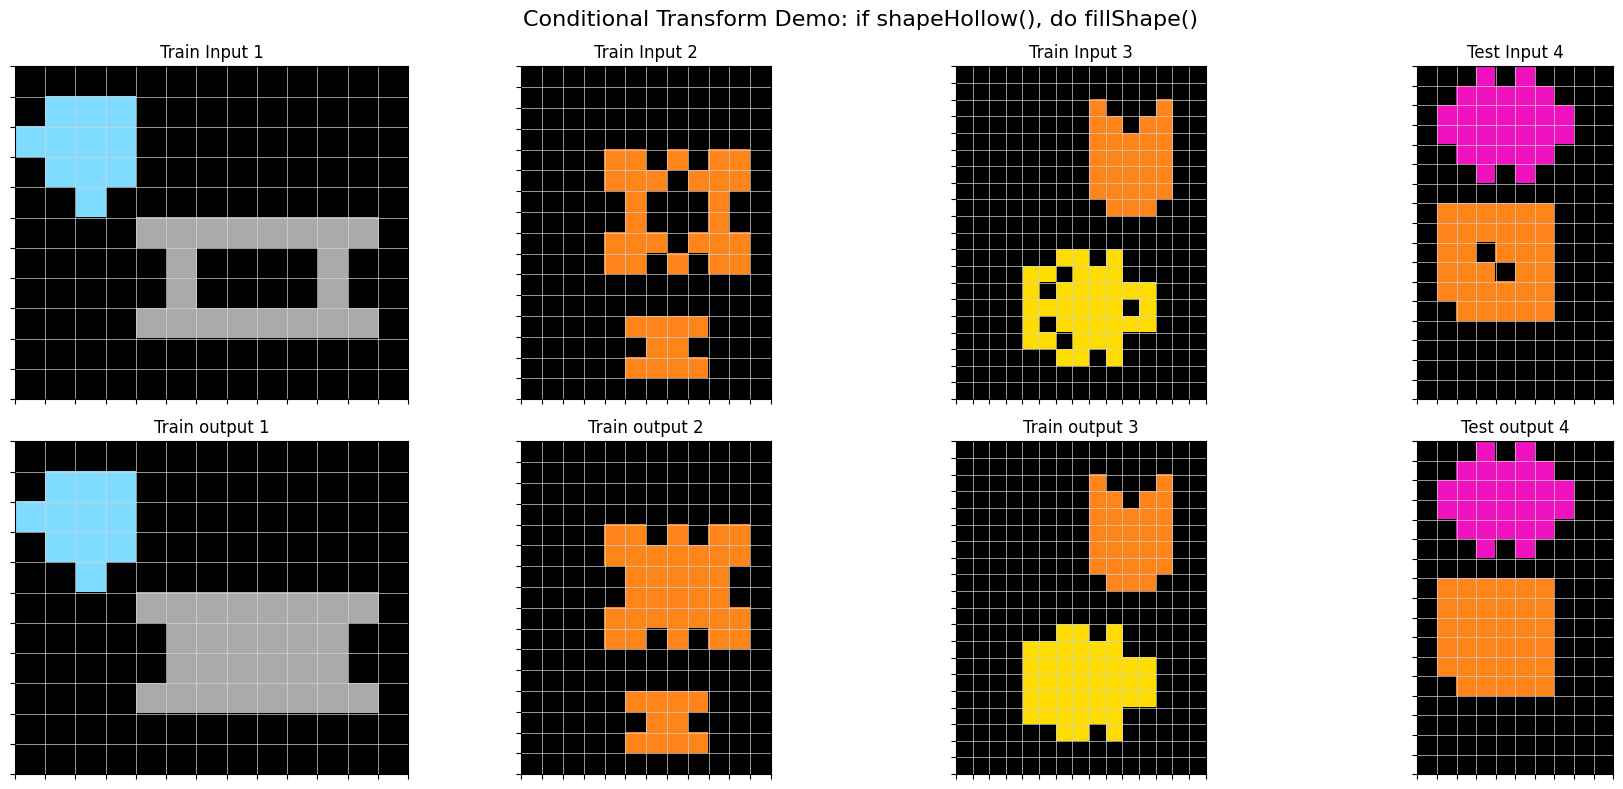
\includegraphics[width=0.8\columnwidth]{Figures/conditional_transfrom_demo_isShapeHollow.png}
    \caption{Simple example of a generated ConditionalTransform schemata task. Fill the hollow object }
    \label{fig:conditional_transform_generated}
\end{figure}

